\section{Theorie}
\label{sec:Theorie}

\subsection{Fehlerrechnung}

Für die Fehlerfortpflanzung bei Gleichungen mit $N$ fehlerbehafteten Größen
wird jeweils die Formel zur Gaußschen Fehlerfortpflanzung

\begin{equation}
  \sigma = \sqrt{\sum_{i=1}^{N}\biggl(\frac{\partial f(x_i)}{\partial x_i}
  \sigma_i\biggr)^2}
\end{equation}
mit der jeweiligen Funktion $f(x_i)$, den Messgrößen $x_i$ und den
zugehörigen Fehlern $\sigma_i$ verwendet.
Zur Berechnung des arithmetischen Mittels von $N$ Messwerten wird jeweils die
Formel

\begin{equation}
  \bar{x} = \frac{1}{N}\sum_{i=1}^{N}x_i
\end{equation}
mit den Messwerten $x_i$ benutzt.
die Standardabweichung des Mittelwerts wird jeweils mit der Gleichung

\begin{equation}
  \bar{\sigma} = \sqrt{\frac{1}{N-1}\sum_{i=1}^{N}(x_i - \bar{x})^2}
\end{equation}
mit den $N$ Messwerten $x_i$ berechnet.

\subsection{Grundlagen}

Der Frequenzbereich des Schalls lässt sich grob in 4 Bereiche einteilen.
Bis ca. \SI{16}{\hertz} wird von Infraschall gesprochen; von ca. 16 bis \SI{20}{\kilo\hertz}
kann der Schall von Menschen gehört werden. Darüber bis ca. \SI{1}{\giga\hertz}
heißt er Ultraschall, mit dem in diesem Versuch gearbeitet wird. Ab ca. \SI{1}{\giga\hertz}
tritt Hyperschall auf.

Nach Formel \eqref{eqn:wellen} ist Schall eine longitudinale Welle und bewegt sich
durch Druckschankungen fort.

\begin{align}
  p(x, t) &= p_0 + v_0 Z \cos(\omega t - k x)\\\label{eqn:wellen}
  \intertext{mit}
  Z &= c \rho \label{eqn:impedanz}
\end{align}

In Bezug auf Reflexion, Brechung und andere Aspekte ähnelt die Schallwelle der
Elektromagnetischen. Allerdings ist sie über $Z$ materialabhängig.
Dabei ist $Z$ die akustische Impedanz beziehungsweise Schallkennwiderstand. $\rho$
ist die Dichte des durchstrahlten Materials und $c$ ist die materialspezifische Schallgeschwindigkeit.
$c$ berechnet sich bei Flüssigkeiten und Gasen, wo nur longitudinale Wellen auftreten
über Formel \eqref{eqn:cfluessig} und bei Festkörpern, bei denen auch Transversalwellen
auftreten über Formel \eqref{eqn:cfest}.

\begin{align}
  c_{\g{Fl}} &= \sqrt{\frac{1}{\kappa \cdot \rho}} \label{eqn:cfluessig}\\
  c_{\g{Fe}} &= \sqrt{\frac{E}{\rho}} \label{eqn:cfest}.
\end{align}

Dabei sind die Schallwellen Richtungsabhängig. Durch Absorption nimmt die Intensität exponentiell ab:

\begin{equation}
  I(x) = I_0 \cdot e^{\alpha x} .
\end{equation}

$\alpha$ ist der Absorptionskoeffizient; er ist beispielweise bei Luft für Ultraschall sehr
niedrig, weshalb bei Untersuchungen mit Ultraschall stets ein Kontaktmitel verwendet werden sollte.

Der Anteil des reflektierten Schalls wird durch den Reflektionskoeffizient $R$ angegeben.
Er wird mit Formel \eqref{eqn:reflexion} berechnet und hängt von den akustischen Impedanzen
$Z_1$ und $Z_2$ der
angrenzenden Materialien ab.

\begin{equation}
  R = (\frac{Z_1 - Z_2}{Z_1 + Z_2})^2
  \label{eqn:reflexion}
\end{equation}

Der Transmittierte Teil ist dann mit $T=1-R$ gegeben.

\subsection{Ultraschall: Erzeugung, Anwendung und Verfahren}

Ultraschall kann durch den \emph{piezo-elektrischen Effekt} erzeugt werden. Dazu wird ein piezoelektrischer
Kristall mit der polaren Achse in Richtung eines elktrischen Feldes plaziert und wird so zur Schwingung
angeregt. In Resonanz können große Schwingungsamplituden erreicht werden.

Außerdem kann der Kristall auch als Empfänger genutzt werden. Dann regt der Schall ihn zur Schwingung an.
Oft werden Quarze verwendet.

In der Medizin wird Ultraschall als Diagnosemittel eingesetzt. Hierzu wird die Laufzeit gemessen.
Das geschieht auf zwei Arten:
Beim Durchschallungsverfahren wird auf der einen Seite des Körpers ein Impuls reingesendet
und auf der anderen Seite mit einem Empfänger aufgenommen. Dann kann anhand der Intensität
gesagt werden, ob sich eine Fehlstelle in dem Körper befindet.
Das Impuls-Echo-Verfahren kann im Gegensatz dazu die Position der Fehlstelle bestimmen.
Hier wird ein Impuls gesendet und dann das reflektierte Signal aufgenommen. Aus
der Laufzeit kann dann nach Formel \eqref{eqn:laufzeit} die Lage bestimmt werden.

%subfigure
\begin{figure}
  \centering
  \begin{subfigure}{0.48\textwidth}
    \centering
    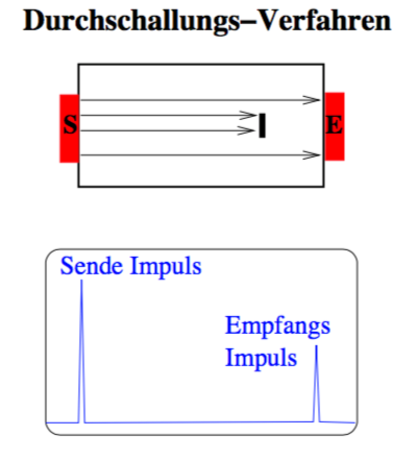
\includegraphics[height=4cm]{Pics/durchschall.pdf}
    \caption{Das Durchschallungsverfahren.}
    \label{fig:durchschall}
  \end{subfigure}
  \begin{subfigure}{0.48\textwidth}
    \centering
    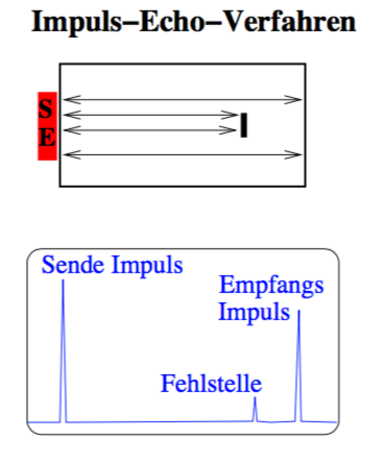
\includegraphics[height=4cm]{Pics/Impuls-Echo.pdf}
    \caption{Das Impuls-Echo-Verfahren.}
    \label{fig:impuls_echo}
  \end{subfigure}
  %\caption{Plot.}
  %\label{fig:plot}
\end{figure}

\begin{equation}
  s = \frac{1}{2} c t
  \label{eqn:laufzeit}
\end{equation}

$c$ ist die Schallgeschwindigkeit.

Die Darstellung der Laufzeitmessung kann anwendungsspezifisch variiert werden.

\begin{itemize}
  \item Der A-Scan (Amplituden Scan) zeigt die Echoamplituden als Funktion der
  Laufzeit in einem eindimesionalen Diagramm.

  \item Der B-Scan (Brightness Scan) zeigt nach dem Bewegen des Senders ein
  zweidimensionales Bild. Die Amplituden werden in unterschiedlichen Farben dargestellt.

  \item Der TM-Scan (Time-Motion Scan) zeigt eine zeitliche Bildfolge. Es sind also hintereinander
  aufgenommene B-Scans.
\end{itemize}


\cite{anleitung}
